
\documentclass[12pt]{article}
\usepackage{amsmath}
\usepackage{amsfonts}
\usepackage{graphicx}
\usepackage{geometry}
\usepackage{float}
\usepackage{caption} 
\geometry{a4paper}
\usepackage{multirow} 
% \geometry{landscape} % rotated page geometry

% See the ``Article customise'' template for come common customisations

\title{Determining the number of clusters of high dimensional vectors via sine matrices and hierarchical agglomerative algorithms}
\author{G.F. Lima}
\date{} % delete this line to display the current date

%%% BEGIN DOCUMENT
\begin{document}

\maketitle
%\tableofcontents

\section{Overview}

Many natural language processing tools, such as Latent Semantic Analysis and word2vec, model a corpus of text as a high dimensional vector space. The semantic similarity between two words can be represented by the cosine of the angle between their respective vector representations. Conversely, one can represent the semantic \emph{distance} by the sine of that angle. Given a list of words $\{ w_1, \ldots, w_n \}$, one can obtain a similarity/distance matrix $M$ such that the entry ${M}_{ij}$  is the similarity/distance between words $w_i$ and $w_j$.

In this paper we shall present a method for finding the number of clusters of a set of high dimensional vectors given their sine matrix.  
%\subsection{}
\section{Variation and distance matrices}

A well known method for determining if two or more groups of data points are significantly distinguishable is to compare the sample variance inside the groups with the sample variance between the groups. In a normed vector space the sample variance is given by
$$
\frac{1}{n-1} \sum_{i = 1}^{i = n} (x_i - \bar{x})^{2},
$$
where $\bar{x}$ is the mean of the $x_i$. A sine matrix will only provide us with a pseudometric on the list of original points, and this might not include their mean, yet given the equation
$$
\sum_{i = 1}^{i = n} (x_i - \bar{x})^{2} = \frac{1}{2n} \sum_{i=1}^n\sum_{j=1}^n (x_i - x_j)^2
$$the sample variance can also be expressed as
$$
\frac{1}{2n(n-1)} \sum_{i=1}^n\sum_{j=1}^n(x_i - x_j)^2.
$$
and the above formula can be generalised to a pseudometric $d$ on the set of points as
$$
\frac{1}{2n(n-1)} \sum_{i=1}^n\sum_{j=1}^nd(x_i, x_j)^2.
$$
Further more, given the usual partition of the total sum of squares as 
$$
\sum_{i=1}^m\sum_{j=1}^{n_i}(x_{ij} - \bar{x})^2 = \sum_{i=1}^m n_i(\bar{x_i} - \bar{x})^2 + \sum_{i=1}^m \sum_{j=1}^{n_i} (x_{ij} - \bar{x_i})^2,
$$
or equivalently
$$
\sum_{i=1}^m n_i(\bar{x_i} - \bar{x})^2 = \sum_{i=1}^m\sum_{j=1}^{n_i}(x_{ij} - \bar{x})^2 - \sum_{i=1}^m\sum_{j=1}^{n_i}(x_{ij} - \bar{x_i})^2
$$
we may generalise the sample variance between groups given by
$$
 \frac{1}{m - 1}\sum_{i=1}^{m} n_i(\bar{x_i} - \bar{x})^2
$$
to
$$
\frac{1}{m-1}\left( \frac{1}{2n}\sum_{i=1}^m\sum_{i^\prime=1}^m\sum_{j=1}^{n_i}\sum_{j^\prime=1}^{n_i}d(x_{ij},x_{i^\prime j^\prime})^2 - \sum_i^{m} \frac{1}{2n_i}\sum_{ j}^{n_i}\sum_{ j^\prime}^{n_i} d(x_{ij}, x_{ij^\prime})^2 \right).
 $$
 From the previous formulas we may generalise the statistic
$$
 \frac{\frac{1}{m-1} \sum_{i=1}^{m} n_i(\bar{x_i} - \bar{x})^2}{\frac{1}{n-m}\sum_i \sum_j (x_{ij} - \bar{x_i})}
 $$
 which is commonly known as the ratio of the between-group variance and the within-group variance, to the following
\begin{equation} \label{varratio}
 \frac{\displaystyle{\frac{1}{m-1}}\left( \displaystyle{ \frac{1}{2n}\sum_{i=1}^m\sum_{i^\prime=1}^m\sum_{j=1}^{n_i}\sum_{j^\prime=1}^{n_i}d(x_{ij},x_{i^\prime j^\prime})^2 - \sum_i^m \frac{1}{2n_i}\sum_{j}^{n_i} \sum_{j^\prime}^{n_i} d(x_{ij}, x_{ij^\prime})^2} \right)}{\displaystyle{\frac{1}{n-m}} \left(\displaystyle{\sum_{i=1}^m \frac{1}{2n_i}\sum_{j=1}^{n_i} \sum_{j^\prime = 1}^{n_i}d(x_{ij}, x_{ij^\prime})} \right)} \tag{$\ast$}
\end{equation}

Let $S$ be a set of $n$ points with metric $d$, and $\mathfrak{S} = \{ S_1, \ldots, S_m \}$ a partition such that, if $i \neq j$, then $S_i \cap S_j = \emptyset$, and $\bigcup S_i = S$. We define the \emph{variation ratio} of $(S, \mathfrak{S}, d)$, or $F(S,\mathfrak{S}, d)$, by the above formula (\ref{varratio}). In this context, given $1 \leq i \leq m$, and $1 \leq j \leq n_i$ the element $x_{ij}$ belongs to the partition $S_i$.  

The reader can probably see that, given a metric space $(S, d)$, a hierarchical clustering algorithm will produce a sequence of partitions $\{\mathfrak{S}_i\}_{i}$ of the original space $S$.

\section{Simulating clusters}\label{sec:simulclstr}
For the purposes of simulating clusters in high dimensions, we shall pick a number $n$ of clusters of size $s$, a natural number $d$ to represent the dimension of the subspace where each will be generated, and a (positive) real number $v$ for the clusters variance. For each $1 \leq i \leq n$ we shall then generate a set $C_i$ of $s$ random vectors following a multivariate normal distribution of $d$ dimensions with mean vector $(1, 1, \ldots, 1)$ and covariance matrix $v \cdot I_d$, where $I_d$ is the identity $d \times d$ matrix.  

To create our sample $S$ of $n$ clusters we shall embed the $C_i$ in an $m$-dimensional space, where $m = n \times s$. 

Let $\iota_k : \mathbb{R}^s \to \mathbb{R}^m$ be the embedding of $\mathbb{R}^s$ into $\mathbb{R}^m$ such that the vector $(x_1, \dots, x_s)$ is mapped to $$(\underbrace{0, \dots, 0}_{k \text{ 0's}}, x_1, \dots, x_s, 0, \dots ).$$

We shall then embed the cluster $C_1$ in to $\mathbb{R}^m$ as $\widehat{C_1} = \iota_0(C_1)$, the cluster $C_2$ as $\widehat{C_2} = \iota_s(C_2)$, and the cluster $C_i$ as $\widehat{C_i} = \iota_{(i-1)s}(C_i)$.  We obtain our sample $S$ by taking the union $\bigcup \widehat{C_i}$.

%Additionally, we might also want some overlap when we embed our clusters into a higher dimensional space. We define the \emph{overlap} factor $\ell$ as a natural number between $0$ and $s$, representing how many dimensions each cluster will share with the next once embedded. Thus, for a sample of overlapping clusters we set $\widehat{C_i} = \iota_{(i - 1)(s - \ell)}(C_i)$.

\section{Variance ratio of samples}

Given a sample of clusters $S$ and a metric $d$, using a hierarchical clustering algorithm we may obtain a finite sequence  $\{ \mathfrak{S}_i \}_{i=1}^N$ of partitions of $S$, and from that a finite sequence of real numbers $\{F(S, \mathfrak{S}_i, d) \}_{i = 1}^N$.

We shall inspect the behaviour of such sequences by looking at 4 different cases, with the same number of clusters, the same sizes of clusters, and the same number of dimensions of the subspaces where they were generated. On all of them we will, for now, set the overlap factor to 0. For each case we will produce twenty different samples $S_1, \ldots, S_{20}$. For each sample $S_j$ we will use an agglomerative single-linkage hierarchical clustering algorithm to produce our sequence of $N$ partitions $\{ \mathfrak{S}_{ji} \}_{i=1}^N$, and, for each $j$, we will plot the function
$$
\begin{array}{rccc}
f_j :&\{1, \ldots, N \} & \to & \mathbb{R} \\
& i & \mapsto & F(S_j, \mathfrak{S}_{ji}, d)
\end{array}
$$ 

The four cases we will look at are:
\begin{itemize}
\item[1.] Two clusters of size 15 generated in subspaces of dimension 10.
\item[2.] Three clusters of size 15 generated in subspaces of dimension 10.
\item[3.] Three clusters of size 15 generated in subspaces of dimension 20.
\item[4.] Four clusters of size 15 generated in subspaces of dimension 10.
\end{itemize}

For the sake of clarity, we have connected the consecutive points $(i, f_j(i))$ and $(i+1, f_j(i+1))$, and so each sample gives us a piece-wise linear function.  The vertical dashed blue line indicates the index $i$ where the hierarchical clustering algorithm produces a partition with the correct number of clusters and the correct sizes. We shall refer to this index as the \emph{target} index.
\begin{figure}[H]
    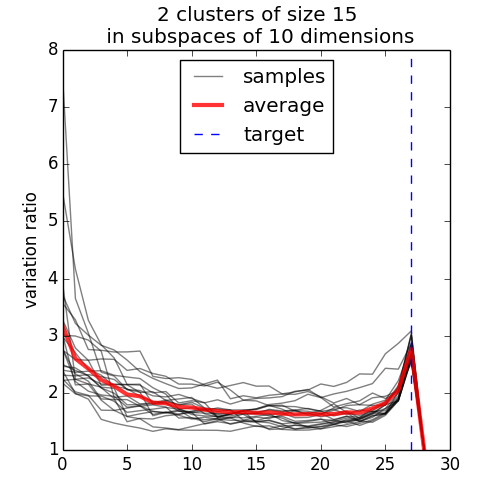
\includegraphics[width=0.50 \textwidth]{2c_s15_sbs10}
    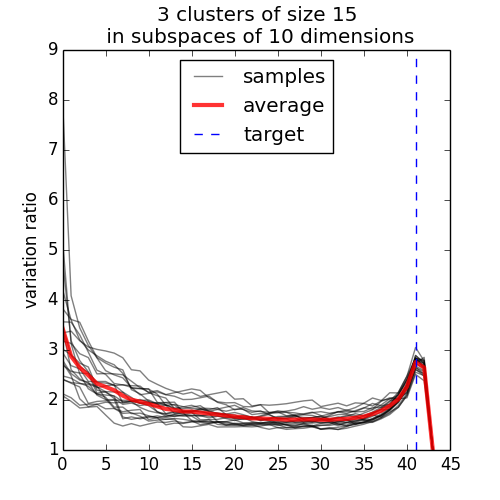
\includegraphics[width=0.50 \textwidth]{3c_s15_sbs10}
    \caption{cases 1 and 2.}
\end{figure}
\begin{figure}[H]
    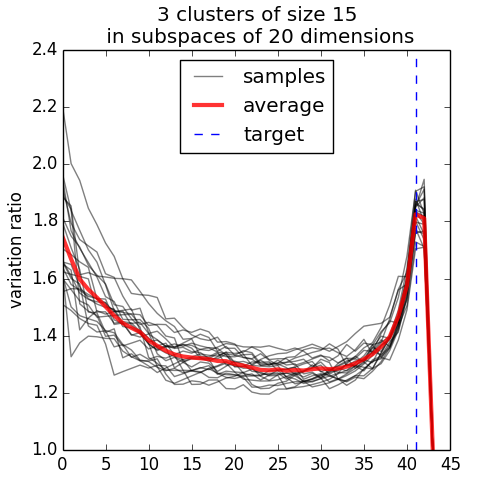
\includegraphics[width=0.50 \textwidth]{3c_s15_sbs20}
    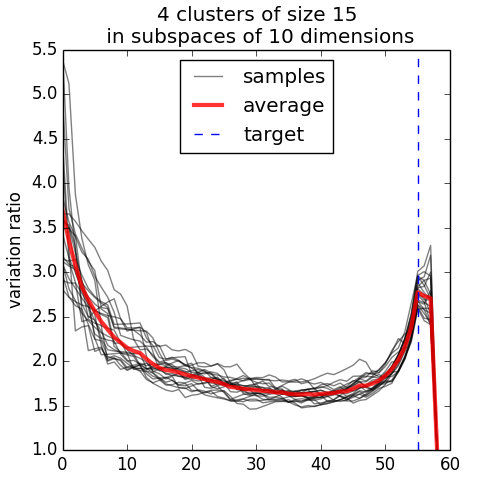
\includegraphics[width=0.50 \textwidth]{4c_s15_sbs10}
    \caption{cases 3 and 4.}
\end{figure}

From the figures we see that the correct partitions coincide with the highest slopes, or more precisely, the target index is where the function
$$
\begin{array}{rccc}
\Delta(f_j) :&\{2, \ldots, N \} & \to & \mathbb{R} \\
& i & \mapsto & f_j(i) - f_j(i-1)
\end{array}
$$ 
obtains its maximum.

%On figures 3 and 4 we can see how the behaviour of $f_j$ changes once we start introducing an overlap factor $\ell > 0.$ Once again, in both figures the coloured lines represent the averages of the values of the $f_j$.
%\begin{figure}[H]
%\centering
%    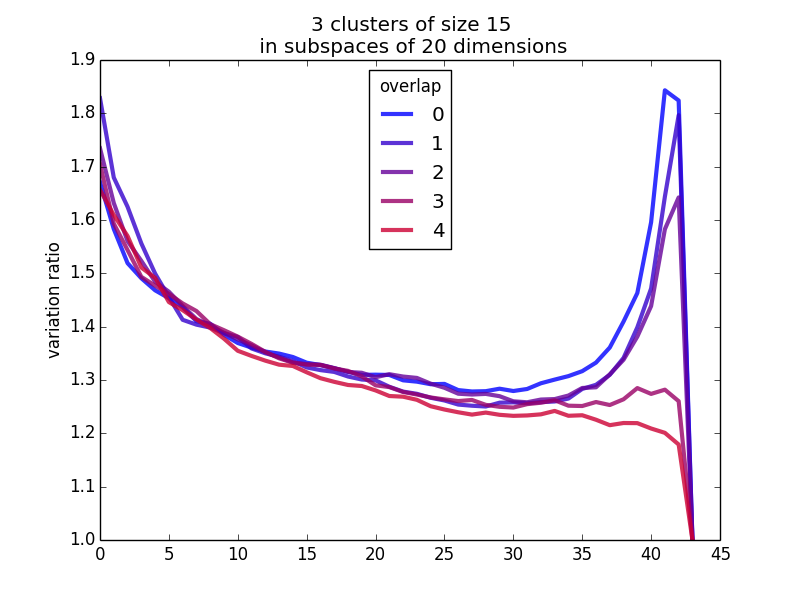
\includegraphics[width=0.80 \textwidth]{3c_s15_sbs20_ovrlp}
%    %\captionsetup[figure]{labelsep=space}
%    \caption{}
%\end{figure}
%\begin{figure}[H]
%\centering
%    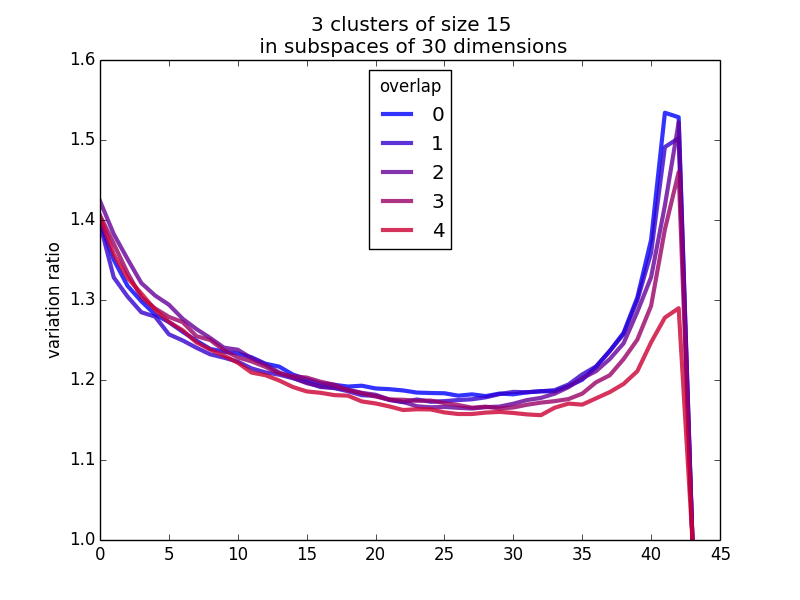
\includegraphics[width=0.80 \textwidth]{3c_s15_sbs30_ovrlp}
%    \caption{}
%\end{figure}

\section{Tests}
\subsection{Multiple clusters}
We fixed the number of clusters, their sizes, and the dimension of the subspaces where they were generated, and then generated 100 different random samples -- as described in section \ref{sec:simulclstr}. The following tables sumarize the prediction accuracy of our algorithm. Each attempt was labeled as correct if it successfully predicted the number of clusters and all their sizes for samples with two, three, four, and five clusters.

\begin{table}[H]
\begin{center}
	\begin{tabular}{cc|c|c|c|}
		\cline{3-5}
		& & \multicolumn{3}{c|}{Size of clusters} \\ 
		\cline{3-5}
		& & 5 & 10 & 15 \\
		\hline
		\multicolumn{1}{|c}{} & 
		\multicolumn{1}{|c|}{5} & 76\% & 87\%& 97\%	 	\\ \cline{2-5}
		\multicolumn{1}{|c}{ subspace} & 
		\multicolumn{1}{|c|}{10} & 85\% & 90\%& 97\% 	\\ \cline{2-5}
		\multicolumn{1}{|c}{ dimension} & 
		\multicolumn{1}{|c|}{15} & 83\% & 99\%& 99\% 	\\ \cline{2-5}
		\multicolumn{1}{|c}{} & 
		\multicolumn{1}{|c|}{20} & 87\% & 99\%& 98\% 	\\ \cline{1-5}
	\end{tabular}
	\caption{Percentage of correct predictions for samples with two clusters.}
	\end{center}
\end{table}

\begin{table}[H]
\begin{center}
	\begin{tabular}{cc|c|c|c|}
		\cline{3-5}
		& & \multicolumn{3}{c|}{Size of clusters} \\ 
		\cline{3-5}
		& & 5 & 10 & 15 \\
		\hline
		\multicolumn{1}{|c}{} & 
		\multicolumn{1}{|c|}{5} & 80\% & 92\%& 89\%	 	\\ \cline{2-5}
		\multicolumn{1}{|c}{ subspace} & 
		\multicolumn{1}{|c|}{10} & 72\% & 90\%& 97\% 	\\ \cline{2-5}
		\multicolumn{1}{|c}{ dimension} & 
		\multicolumn{1}{|c|}{15} & 82\% & 90\%& 100\% 	\\ \cline{2-5}
		\multicolumn{1}{|c}{} & 
		\multicolumn{1}{|c|}{20} & 77\% & 96\%& 96\% 	\\ \cline{1-5}
	\end{tabular}
	\caption{Percentage of correct predictions for samples with three clusters.}
\end{center}
\end{table}

\begin{table}[H]
\begin{center}
	\begin{tabular}{cc|c|c|c|}
		\cline{3-5}
		& & \multicolumn{3}{c|}{Size of clusters} \\ 
		\cline{3-5}
		& & 5 & 10 & 15 \\
		\hline
		\multicolumn{1}{|c}{} & 
		\multicolumn{1}{|c|}{5} & 71\% & 87\%& 87\%	 	\\ \cline{2-5}
		\multicolumn{1}{|c}{ subspace} & 
		\multicolumn{1}{|c|}{10} & 72\% & 83\%& 99\% 	\\ \cline{2-5}
		\multicolumn{1}{|c}{ dimension} & 
		\multicolumn{1}{|c|}{15} & 76\% & 90\%& 95\% 	\\ \cline{2-5}
		\multicolumn{1}{|c}{} & 
		\multicolumn{1}{|c|}{20} & 60\% & 91\%& 98\% 	\\ \cline{1-5}
	\end{tabular}
	\caption{Percentage of correct predictions for samples with four clusters.}
\end{center}
\end{table}

\begin{table}[H]
\begin{center}
	\begin{tabular}{cc|c|c|c|}
		\cline{3-5}
		& & \multicolumn{3}{c|}{Size of clusters} \\ 
		\cline{3-5}
		& & 5 & 10 & 15 \\
		\hline
		\multicolumn{1}{|c}{} & 
		\multicolumn{1}{|c|}{5} & 68\% & 82\%& 90\%	 	\\ \cline{2-5}
		\multicolumn{1}{|c}{ subspace} & 
		\multicolumn{1}{|c|}{10} & 50\% & 84\%& 98\% 	\\ \cline{2-5}
		\multicolumn{1}{|c}{ dimension} & 
		\multicolumn{1}{|c|}{15} & 61\% & 88\%& 99\% 	\\ \cline{2-5}
		\multicolumn{1}{|c}{} & 
		\multicolumn{1}{|c|}{20} & 48\% & 90\%& 95\% 	\\ \cline{1-5}
	\end{tabular}
	\caption{Percentage of correct predictions for samples with five clusters.}
\end{center}
\end{table}

\subsection{Single cluster samples}

For samples with only a single cluster, the algorithm exhibits a significantly lower accuracy, as the following table can show.

\begin{table}[H]
\begin{center}
	\begin{tabular}{cc|c|c|c|}
		\cline{3-5}
		& & \multicolumn{3}{c|}{Size of clusters} \\ 
		\cline{3-5}
		& & 5 & 10 & 15 \\
		\hline
		\multicolumn{1}{|c}{} & 
		\multicolumn{1}{|c|}{5} & 14\% & 0\%& 0\%	 	\\ \cline{2-5}
		\multicolumn{1}{|c}{ subspace} & 
		\multicolumn{1}{|c|}{10} & 7\% & 0\%& 0\% 	\\ \cline{2-5}
		\multicolumn{1}{|c}{ dimension} & 
		\multicolumn{1}{|c|}{15} & 5\% & 0\%& 0\% 	\\ \cline{2-5}
		\multicolumn{1}{|c}{} & 
		\multicolumn{1}{|c|}{20} & 4\% & 0\%& 0\% 	\\ \cline{1-5}
	\end{tabular}
	\caption{Percentage of correct predictions for samples with a single cluster.}
\end{center}
\end{table}
This is due to the fact that the between-group variance is zero when there is only one partition of $S$, yet this partition represents the correct number of clusters. One could say that this case is outside the scope of our algorithm, since our variation ratio presuposes more than one group of points. 

In practice, what happens is that our algorithm indicates a cut off index  smaller than the correct one, and, since we are using an aglomerative clustering algorithm, it yields the single cluster split into multiple parts which haven't yet been aglomerated.  

%\subsection{Merging subspaces}
%\subsubsection{Single linkage method}
%Using single linkage method, all clusters with size 15.

%\begin{table}[H]
%\begin{center}
%	\begin{tabular}{cc|c|c|c|c|}
%		\cline{3-6}
%		& & \multicolumn{4}{c|}{Merge factor} \\ 
%		\cline{3-6}
%		& & 1 & 2 & 3 & 4 \\
%		\hline
%		\multicolumn{1}{|c}{} & 
%		\multicolumn{1}{|c|}{5} & 33\% & 22\%& 13\% & 16\%	 	\\ \cline{2-6}
%		\multicolumn{1}{|c}{ subspace} & 
%		\multicolumn{1}{|c|}{10} &68\% & 23\%& 21\% & 21\%	\\ \cline{2-6}
%		\multicolumn{1}{|c}{ dimension} & 
%		\multicolumn{1}{|c|}{15} & 75\% & 35\%& 24\% & 17\%	\\ \cline{2-6}
%		\multicolumn{1}{|c}{} & 
%		\multicolumn{1}{|c|}{20} & 85\% & 60\%& 42\% & 32\%	\\ \cline{1-6}
%	\end{tabular}
%	\caption{Percentage of correct predictions for samples with two clusters.}
%\end{center}
%\end{table}

%\begin{table}[H]
%\begin{center}
%	\begin{tabular}{cc|c|c|c|c|}
%		\cline{3-6}
%		& & \multicolumn{4}{c|}{Merge factor} \\ 
%		\cline{3-6}
%		& & 1 & 2 & 3 & 4 \\
%		\hline
%		\multicolumn{1}{|c}{} & 
%		\multicolumn{1}{|c|}{5} & 19\% & 15\%& 14\% & 12\%	 	\\ \cline{2-6}
%		\multicolumn{1}{|c}{ subspace} & 
%		\multicolumn{1}{|c|}{10} &34\% & 20\%& 20\% & 18\%	\\ \cline{2-6}
%		\multicolumn{1}{|c}{ dimension} & 
%		\multicolumn{1}{|c|}{15} & 52\% & 30\%& 23\% & 20\%	\\ \cline{2-6}
%		\multicolumn{1}{|c}{} & 
%		\multicolumn{1}{|c|}{20} & 61\% & 44\%& 21\% & 23\%	\\ \cline{1-6}
%	\end{tabular}
%	\caption{Percentage of correct predictions for samples with three clusters.}
%\end{center}
%\end{table}

%\begin{table}[H]
%\begin{center}
%	\begin{tabular}{cc|c|c|c|c|}
%		\cline{3-6}
%		& & \multicolumn{4}{c|}{Merge factor} \\ 
%		\cline{3-6}
%		& & 1 & 2 & 3 & 4 \\
%		\hline
%		\multicolumn{1}{|c}{} & 
%		\multicolumn{1}{|c|}{5} & 10\% & 9\%& 17\% & 10\%	 	\\ \cline{2-6}
%		\multicolumn{1}{|c}{ subspace} & 
%		\multicolumn{1}{|c|}{10} &16\% & 18\%& 16\% & 13\%	\\ \cline{2-6}
%		\multicolumn{1}{|c}{ dimension} & 
%		\multicolumn{1}{|c|}{15} & 38\% & 11\%& 17\% & 14\%	\\ \cline{2-6}
%		\multicolumn{1}{|c}{} & 
%		\multicolumn{1}{|c|}{20} & 60\% & 25\%& 17\% & 24\%	\\ \cline{1-6}
%	\caption{Percentage of correct predictions for samples with four clusters.}
%\end{center}
%\end{table}

%\begin{table}[H]
%\begin{center}
%	\begin{tabular}{cc|c|c|c|c|}
%		\cline{3-6}
%		& & \multicolumn{4}{c|}{Merge factor} \\ 
%		\cline{3-6}
%		& & 1 & 2 & 3 & 4 \\
%		\hline
%		\multicolumn{1}{|c}{} & 
%		\multicolumn{1}{|c|}{5} & 8\% & 14\%& 9\% & 6\%	 	\\ \cline{2-6}
%		\multicolumn{1}{|c}{ subspace} & 
%		\multicolumn{1}{|c|}{10} &9\% & 12\%& 13\% & 14\%	\\ \cline{2-6}
%		\multicolumn{1}{|c}{ dimension} & 
%		\multicolumn{1}{|c|}{15} & 25\% & 8\%& 10\% & 12\%	\\ \cline{2-6}
%		\multicolumn{1}{|c}{} & 
%		\multicolumn{1}{|c|}{20} & 43\% & 10\%& 8\% & 7\%	\\ \cline{1-6}
%	\end{tabular}
%	\caption{Percentage of correct predictions for samples with five clusters.}
%\end{center}
%\end{table}

%\subsubsection{Complete linkage method}

%Using complete linkage method, all clusters with size 15.
%
%\begin{table}[H]
%\begin{center}
%	\begin{tabular}{cc|c|c|c|c|}
%		\cline{3-6}
%		& & \multicolumn{4}{c|}{Merge factor} \\ 
%		\cline{3-6}
%		& & 1 & 2 & 3 & 4 \\
%		\hline
%		\multicolumn{1}{|c}{} & 
%		\multicolumn{1}{|c|}{5} & 48\% & 26\%& 23\% & 20\%	 	\\ \cline{2-6}
%		\multicolumn{1}{|c}{ subspace} & 
%		\multicolumn{1}{|c|}{10} &62\% & 38\%& 46\% & 20\%	\\ \cline{2-6}
%		\multicolumn{1}{|c}{ dimension} & 
%		\multicolumn{1}{|c|}{15} & 61\% & 53\%& 44\% & 37\%	\\ \cline{2-6}
%		\multicolumn{1}{|c}{} & 
%		\multicolumn{1}{|c|}{20} & 69\% & 61\%& 50\% & 36\%	\\ \cline{1-6}
%	\end{tabular}
%	\caption{Percentage of correct predictions for samples with two clusters.}
%\end{center}
%\end{table}
%
%\begin{table}[H]
%\begin{center}
%	\begin{tabular}{cc|c|c|c|c|}
%		\cline{3-6}
%		& & \multicolumn{4}{c|}{Merge factor} \\ 
%		\cline{3-6}
%		& & 1 & 2 & 3 & 4 \\
%		\hline
%		\multicolumn{1}{|c}{} & 
%		\multicolumn{1}{|c|}{5} & 23\% & 4\%& 18\% & 14\%	 	\\ \cline{2-6}
%		\multicolumn{1}{|c}{ subspace} & 
%		\multicolumn{1}{|c|}{10} &29\% & 14\%& 5\% & 5\%	\\ \cline{2-6}
%		\multicolumn{1}{|c}{ dimension} & 
%		\multicolumn{1}{|c|}{15} & 42\% & 25\%& 8\% & 10\%	\\ \cline{2-6}
%		\multicolumn{1}{|c}{} & 
%		\multicolumn{1}{|c|}{20} & 43\% & 21\%& 21\% & 9\%	\\ \cline{1-6}
%	\end{tabular}
%	\caption{Percentage of correct predictions for samples with three clusters.}
%\end{center}
%\end{table}
%
%\begin{table}[H]
%\begin{center}
%	\begin{tabular}{cc|c|c|c|c|}
%		\cline{3-6}
%		& & \multicolumn{4}{c|}{Merge factor} \\ 
%		\cline{3-6}
%		& & 1 & 2 & 3 & 4 \\
%		\hline
%		\multicolumn{1}{|c}{} & 
%		\multicolumn{1}{|c|}{5} & 16\% & 8\%& 0\% & 8\%	 	\\ \cline{2-6}
%		\multicolumn{1}{|c}{ subspace} & 
%		\multicolumn{1}{|c|}{10} &19\% & 15\%& 12\% & 13\%	\\ \cline{2-6}
%		\multicolumn{1}{|c}{ dimension} & 
%		\multicolumn{1}{|c|}{15} & 28\% & 20\%& 21\% & 11\%	\\ \cline{2-6}
%		\multicolumn{1}{|c}{} & 
%		\multicolumn{1}{|c|}{20} & 26\% & 21\%& 13\% & 11\%	\\ \cline{1-6}
%	\end{tabular}
%	\caption{Percentage of correct predictions for samples with four clusters.}
%\end{center}
%\end{table}
%
%\begin{table}[H]
%\begin{center}
%	\begin{tabular}{cc|c|c|c|c|}
%		\cline{3-6}
%		& & \multicolumn{4}{c|}{Merge factor} \\ 
%		\cline{3-6}
%		& & 1 & 2 & 3 & 4 \\
%		\hline
%		\multicolumn{1}{|c}{} & 
%		\multicolumn{1}{|c|}{5} & 13\% & 16\%& 8\% & 11\%	 	\\ \cline{2-6}
%		\multicolumn{1}{|c}{ subspace} & 
%		\multicolumn{1}{|c|}{10} &29\% & 20\%& 17\% & 8\%	\\ \cline{2-6}
%		\multicolumn{1}{|c}{ dimension} & 
%		\multicolumn{1}{|c|}{15} & 20\% & 15\%& 12\% & 13\%	\\ \cline{2-6}
%		\multicolumn{1}{|c}{} & 
%		\multicolumn{1}{|c|}{20} & 21\% & 17\%& 19\% & 10\%	\\ \cline{1-6}
%	\end{tabular}
%	\caption{Percentage of correct predictions for samples with five clusters.}
%\end{center}
%\end{table}
\section{Conclusion}

The algorithm presents good predictive power for samples of 2 clusters or more where the clusters occur in distinct dimensions.
\end{document}